\chapter{Introduction}
\label{chap:intro}


\section{Motivation}

% Introduction, Objective
%  Why is it important, 
% what is the problem, 
This report presents a comprehensive exploration of various LiDAR-based place recognition algorithms focusing on their application in long-term navigation across unstructured natural environments. 
Place recognition is the capability to identify specific revisited locations and correctly determining robot's pose by comparing the current observation with previously visited places. 

The primary goal is to design and integrate a LiDAR place recognition system within a Simultaneous Localization and Mapping (SLAM) framework. 
This integration is key for achieving robust loop closure detection, precise pose optimization, and the creation of accurate 3D maps, which are essential for long-term navigation and mapping systems.

% What is place recognition
% Motivation 
% Why LiDAR 
In context of long-term navigation, LiDAR proves to be more robust than RGB cameras, capable of capturing much longer-range 3D scene data,  less susceptible to estricted viewpoints and visual change due to lighting conditions.
Therefore, LiDAR is used as a main sensor to obtain 3D pointclouds of the environment, then processing 3D pointclouds to extract meaningful features to check previously visited places.

% LiDAR place recognition methods
% 1. Handcrafted features
% 2. Learning-based features
Descritors are used to represent the environment and compare with each other to determine whether the current observation is a revisited place.
There are two main approaches: handcrafted features and learning-based features.
Handcrafted features are manually designed to capture the geometric characteristics of the environment.
This approach is more generalizable and robust to changes in the environment, but it is difficult to design features that are both discriminative and invariant to environmental changes.
Recently, learning-based features using recent deep-learning became popular in place recognition.

\section{Challenges in natural environments}
% Why natural environment 
Despite the advantages of LiDAR in place recognition, its application in unstructured natural environments like forests presents several notable challenges.
Firstly, the task of extracting meaningful features from 3D point clouds in these settings is complex. 
Natural environments are irregular structures like trees, which not only lack fine structure but also undergo seasonal changes, affecting their shape and density over time. 
This complicates the creation of consistent geometric representations crucial for accurate place recognition.
Secondly, the limitation in the LiDAR's field of view poses a significant challenge. In large-scale natural environment, LiDAR sensors often struggle to capture the complete vertical extent of the environment. 
This issue is particularly pronounced in areas with tall trees or undulating terrain, where the full scope of the environment is crucial for comprehensive mapping and navigation.
Thirdly, processing the voluminous 3D data typical of LiDAR systems, such as point clouds, demands substantial computational resources in terms of memory and processing time. 
This requirement poses a considerable challenge for robotic applications, where often limited computational resources are available, and real-time performance is essential.
Lastly, the dynamic nature of unstructured terrains contrasts sharply with the more predictable environments of urban or structured settings, like roads used in autonomous driving. 
In natural landscapes, the paths and terrains are subject to continual change. 
The extreme orientation and movement often encountered in unstructured environments can lead to sparse and unreliable sensor data, exacerbating the issue of frequent odometry drift.

\begin{figure}[h]
\centering  
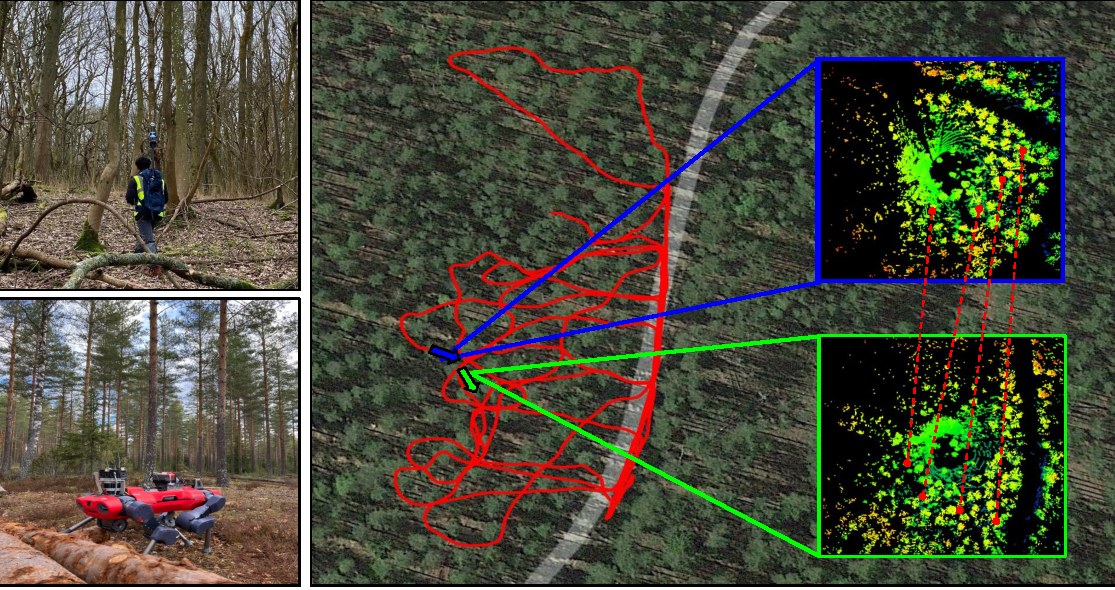
\includegraphics[width=0.99\textwidth]{pics/intro_motivation_fig_189_100}    
\caption{Place recognition in dense forest environments using a backpack-mounted LiDAR and legged robot equipped with LiDAR.
Right: Illustration of loop closure detection within a deeply forested area, with a baseline distance of xx meters and an orientation offset of yy degrees. Dotted red lines highlight corresponding locations from the two point clouds.}
\label{fig:intro_motivation}
\end{figure}

% Contribution 
\section{Contribution}
Overall, there is a compelling need for LiDAR place recognition in natural environments. 
In this report, I showed
\begin{itemize}
\item 1. Evaluation of both handcrafted and learning-based LiDAR place recognition models' descriptors in dense forest environments.

\item 2. Complete pipeline integrating loop closures into a SLAM system.

\item 3. Analysis of loop-closure pairs based on distances and viewpoints differences.

\item 4. Demonstration of our system for online and offline SLAM modes, as well as relocalization in previously mapped mapped environments. 

\end{itemize}
% \section{Motivation}

% Legged robots have the potential to perform tasks that are extremely challenging or risky for humans, such as exploration of unknown locations or rescue operations. The recent \gls{darpa} SubT challenge (2018-2021) was a clear demonstration of the advantages of such platforms for exploration in urban and underground environments~\cite{Ackerman2022}. When the challenge started in 2018, 3 out of 11 teams were using legged robots for the competition; 3 years later almost every team relied on them as their core platforms~\cite{Chung2023}. Their versatility when negotiating different kinds of terrain compared to wheeled robots, as well as their increased payload capabilities compared to aerial ones offer a good balance for their deployment in the field.

% A key aspect of this success has been the impressive mobility skills achieved by the locomotion controllers developed by the research community over the last few years~\cite{Gangapurwala2020, Miki2022a, Kumar2021}, combined with the consolidation of commercial platforms such as the Boston Dynamics' Spot~\cite{BostonDynamics} and ANYbotics' ANYmal~\cite{Anybotics} quadrupeds, and humanoids such as the Agility Robotics' Digit~\cite{AgilityRobotics}. This offers an unprecedented scenario for their mass adoption in applications such as last-mile delivery, industrial inspection, monitoring, or rescue.

% The new locomotion controllers have unlocked new environments where legged robots can operate: not only warehouses with flat terrain but also industrial environments with complex staircases~\cite{BostonDynamics}, urban and disaster scenarios~\cite{Lee2020}, underground environments~\cite{Miki2022a}, as well as natural scenes such as forests and grasslands~\cite{Kumar2021}. However, this comes with new challenges: while legged robots \emph{can now walk} on challenging terrain, this does not necessarily guarantee that they can \emph{execute autonomous missions} in such environments. For example, a legged robot might have the capacity to walk up a staircase given by its hardware design and locomotion control, but if a motion planner does not consider staircases as valid planning areas such advanced capabilities are futile. 

% As a consequence, moving from low-level locomotion problems to higher-level tasks such as navigation and mission planning is one of the main research challenges for legged robotics nowadays~\cite{Wellhausen2022}.

% \begin{figure}[t]
% 	\centering
% 	\includegraphics[width=\textwidth]{figures/motivation/motivation.jpg}
% 	\caption{Autonomous deployments of legged robots using the contributions presented in this thesis. They include industrial environments, underground mines, public parks, and forests.}
% 	\label{fig:motivation}
% \end{figure}

% \section{Objective}
% The main objective of this thesis is to develop new navigation systems for legged robots. We define navigation as the problem of safely moving between two locations A and B while avoiding obstacles and other risky areas~\cite{Corke2011,Lynch2017,Ekstrom2018}. While the definition is concise, developing such capabilities for robotic systems is a complex problem that requires a strong coordination of perception, planning, and control methods.

% The second objective is then to develop the specific systems and methods that, when seamlessly integrated, enable legged robot navigation.

% Last, we aim to achieve navigation in challenging environments: spaces that can be dynamic, difficult to access by humans, or simply risky. Specific examples include  industrial facilities, mines, tunnels, or open natural scenes.

% %In this work we present three solutions for this purpose. They address localisation, scene understanding and local planning with legged platforms. These have been tested onboard, in closed-loop, demonstrating real-world navigation in environments such as structured industrial facilities, underground mines, and forests, .

% \section{Contributions}
% The main contribution of this thesis is the investigation, implementation, and field deployment of new navigation systems to expand the use of legged robots in challenging environments, as shown in \figref{fig:motivation}. The systems were designed to be simple but principled, exploiting fundamental ideas of optimisation methods as well as the constraints and advantages that legged robots present.

% The specific contributions of this work include:
% \begin{itemize}[leftmargin=*]
% 	\item An entropy-based approach for active camera selection that robustifies multi-camera localisation systems under transient scene changes.
% 	\item A local planning system that relies on local scene representations to achieve safe and reactive navigation.
% 	\item A framework for self-supervised online traversability learning that enables fast deployment in unknown environments.
% 	\item A mission planning system for autonomous forest inventory with legged robots.
% 	\item Hardware integration and deployment of these systems on legged platforms in industrial, underground, and natural environments.
% \end{itemize}


% \section{Publications}
% \label{sec:thesis-publications}
% The previous contributions have been materialised through three first-author peer-reviewed publications developed during this project. Additional contributions include six non-first-author peer-reviewed articles. Other open-source packages and tutorials are listed in \appref{app:A}. 

% \subsection{First-author Publications}
% \begin{enumerate}[leftmargin=*]
% 	\item \highlight{Mattamala, M.}, Ramezani, Camurri, M., Fallon, M. (2021). Learning Camera Performance Models for Active Multi-Camera Visual Teach and Repeat. \emph{IEEE International Conference on Robotics and Automation (ICRA)}. \cite{Mattamala2021}
% 	%
% 	\item \highlight{Mattamala, M.}, Chebrolu, N., Fallon, M. (2022). An Efficient Locally Reactive Controller for Safe Navigation in Visual Teach and Repeat Missions. \emph{IEEE Robotics and Automation Letters (RA-L)}. \cite{Mattamala2022}
% 	%
% 	\item Frey, J.*, \highlight{Mattamala, M.}*, Chebrolu, N., Cadena, C., Fallon, M., Hutter, M. (2023). Fast Traversability Estimation for Wild Visual Navigation. \emph{Robotics: Science and Systems}. \cite{Frey2023} (*equal contribution.)
% \end{enumerate}

% % \subsection{Draft}
% % \begin{enumerate}[leftmargin=*]
% % 	\item \highlight{Mattamala, M.}, Frey, J., Chebrolu, N., Casseau, B., Tuna, T., Cadena, C., Hutter, M., Fallon, M. (2023) Conceptualization and Field Deployment of a Legged Forest Ranger Robot. \emph{In preparation}. 
% % \end{enumerate}

% \subsection{Co-authored Publications}
% \begin{enumerate}[leftmargin=*]
%     \item Ramezani, M., Wang, Y., Camurri, M., Wisth, D., \highlight{Mattamala, M.}, Fallon, M. (2020). The Newer College Dataset: Handheld LiDAR, Inertial and Vision with Ground Truth. \emph{IEEE/RSJ International Conference on Intelligent Robots and Systems (IROS)}. \cite{Ramezani2020b}
%     %
% 	\item Wang, Y., Ramezani, M., \highlight{Mattamala, M.}, Fallon, M. (2021). Scalable and Elastic LiDAR Reconstruction in Complex Environments Through Spatial Analysis. \emph{European Conference on Mobile Robots (ECMR)}. \cite{Wang2021}
% 	%
% 	\item Ramezani, M., \highlight{Mattamala, M.}, Fallon, M. (2022). AEROS: Adaptive RObust least-Squares for Graph-Based SLAM. \emph{Frontiers in Robotics and AI}. \cite{Ramezani2022}
% 	%
% 	\item Wang, Y., Ramezani, M., \highlight{Mattamala, M.}, Digumarti, T., Fallon, M. (2022). Strategies for Large Scale Elastic and Semantic LiDAR Reconstruction. \emph{Robotics and Autonomous Systems}. \cite{Wang2022}
% 	%
% 	\item Tranzatto, M., Dharmadhikari, M., Bernreiter, \etal{}, including \highlight{Mattamala, M.} 
%     %L., Camurri, M., Khattak, S., Mascarich, F., Pfreundschuh, P., Wisth, D., Zimmermann, S., Kulkarni, M., Reijgwart, V., Casseau, B., Homberger, T., Petris, P.D., Ott, L., Tubby, W., Waibel, G., Nguyen, H., Cadena, C., Buchanan, R., Wellhausen, L., Khedekar, N., Andersson, O., Zhang, L., Miki, T., Dang, T., \highlight{Mattamala, M.}, Montenegro, M., Meyer, K., Wu, X., Briod, A., Mueller, M.W., Fallon, M.F., Siegwart, R.Y., Hutter, M., Alexis, K. 
%     (2023). Team CERBERUS Wins the DARPA Subterranean Challenge: Technical Overview and Lessons Learned. \emph{Field Robotics}. \cite{Tranzatto2023}
% 		%
% 	\item Erni, G., Frey, J., Miki, T., \highlight{Mattamala, M.}, Hutter, M (2023).  MEM: Multi-Modal Elevation Mapping for Robotics and Learning. \emph{IEEE/RSJ International Conference on Intelligent Robots and Systems (IROS)}.
% \end{enumerate}

% \section{Thesis Outline}
% This thesis is presented in the \emph{integrated format} of the University of Oxford. Chapters 4-6 consist of peer-reviewed publications, each one accompanied by additional discussion as well as a Statement of Authorship declaring the author's contribution to each work. Chapter 7 is an original chapter describing a real-world application.

% The remainder of the thesis is structured as follows:
% \begin{itemize}[leftmargin=*]
% 	%\item \textbf{Chapter 1 -- Introduction:} The present chapter, summarising the objectives, contributions, and achievements.
% 	\item \textbf{Chapter 2 -- Background:} Presentation of the main definitions, theory, and methods used in the thesis.
% 	\item \textbf{Chapter 3 - Related Work:} Review of the relevant literature on robot navigation, with a particular focus on legged platforms.
% 	\item \textbf{Chapter 4 -- Multi-camera Visual Localisation:} An approach to reliably localising robots by actively choosing the \emph{most informative} camera during deployment.
% 	\item \textbf{Chapter 5 -- Reactive Local Planning:} How to navigate in challenging, narrow environments using a reactive local planning approach.
% 	\item \textbf{Chapter 6 -- Online Traversability Learning:} Overcoming the challenges of data collection and curation in traversability estimation via online self-supervised learning.
% 	\item \textbf{Chapter 7 -- Autonomous Forest Inventory:} Conceptualisation and field deployment of autonomous legged robots for forestry applications.
% 	\item \textbf{Chapter 8 -- Conclusion:} Discussion on the achievements and limitations of this work, lessons learned, and future directions for the field.
% \end{itemize}